% ----------------------------------------------------------
% Apêndices
% ----------------------------------------------------------

% ---
% Inicia os apêndices
% ---
\begin{apendicesenv}

% Imprime uma página indicando o início dos apêndices
\partapendices

\chapter{Imagem do circuito para a representação de um número de 4 \textit{bits} em um display de 7 segmentos}
	\label{apendice:CircuitoEtapa1}
	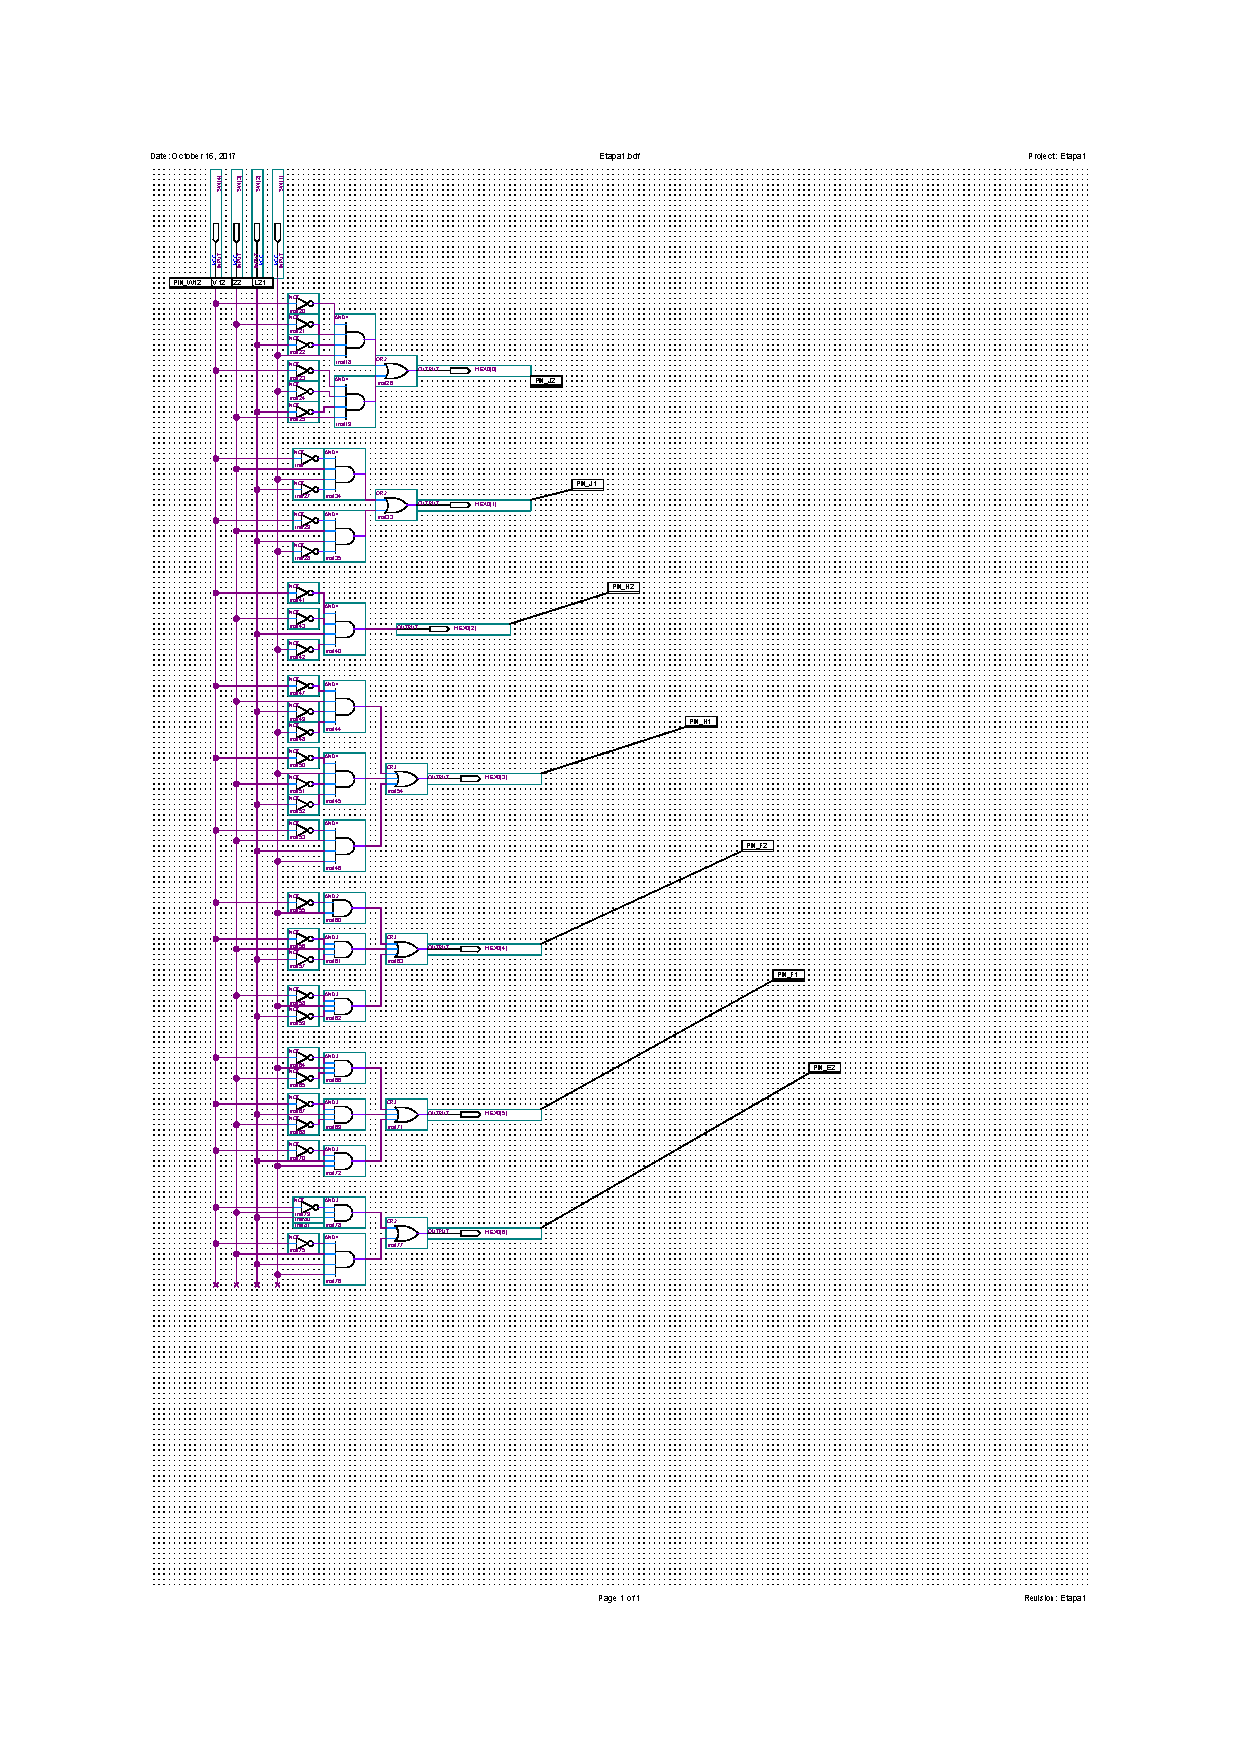
\includepdf[pages=1,frame=false]{apendices/CircuitoSegmentos7.pdf}

	\chapter{Circuito do meio-somador de um 1 \textit{bit}}
		\label{apendice:CircuitoEtapa2}
		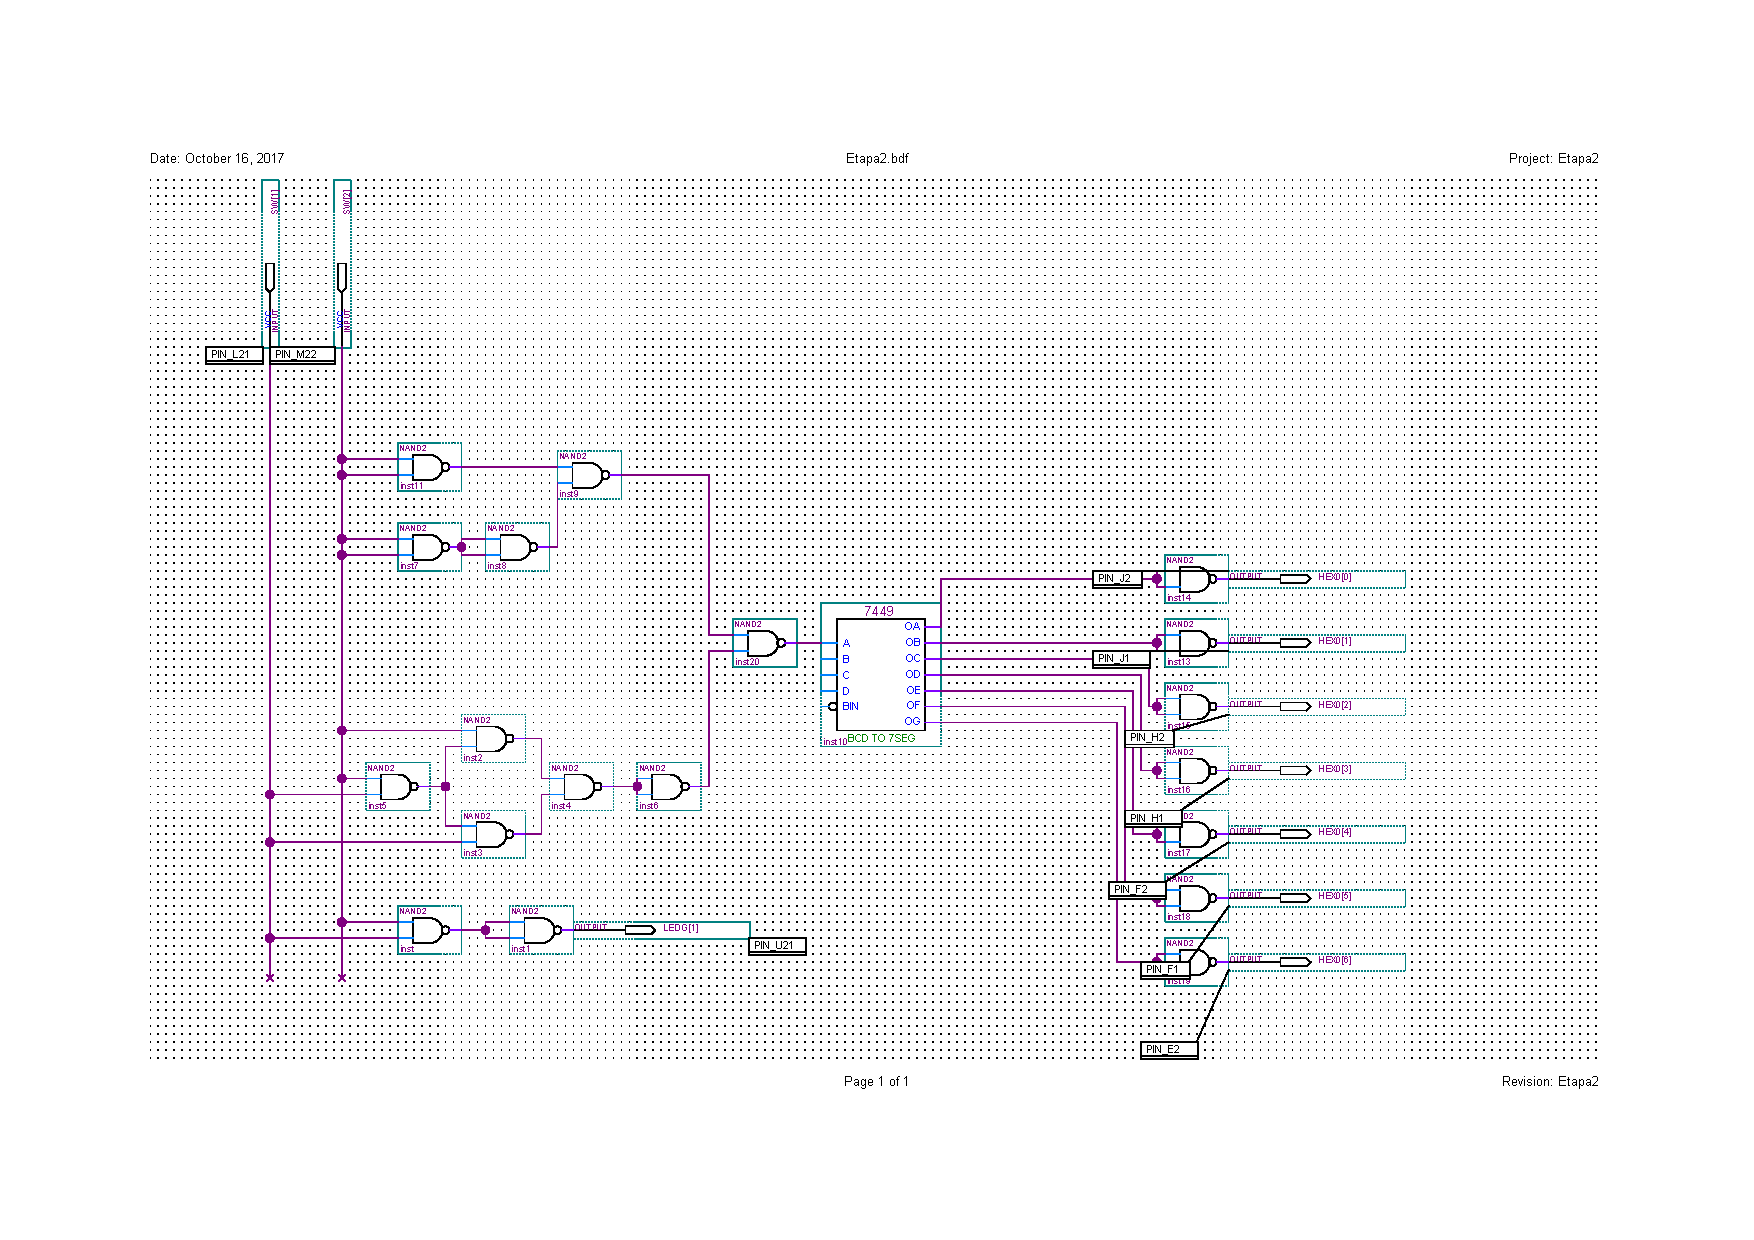
\includepdf[pages=1,landscape,frame=false]{apendices/CircuitoMeioSomador1Bit.pdf}

		Nota: Este diagrama esquemático, diferente do anterior, já foi feito
		utilizando exclusivamente portas NAND, não sendo necessária qualquer metodologia de conversão.
		O circuito utilizado, o TTL 7449\footnote{Para mais detalhes sobre o TTL 7449 acesse o \autoref{anexo:datasheet-7449}.}, apenas substitui aqui o circuito criado para a implementação
		da etapa anterior, respeitando as expressões do item 2.1. É só um circuito já conhecido que
		cumpre a mesma função que o que foi criado para aquela etapa do experimento.

\chapter{Imagem do circuito do meio-somador de 4 \textit{bits}}
	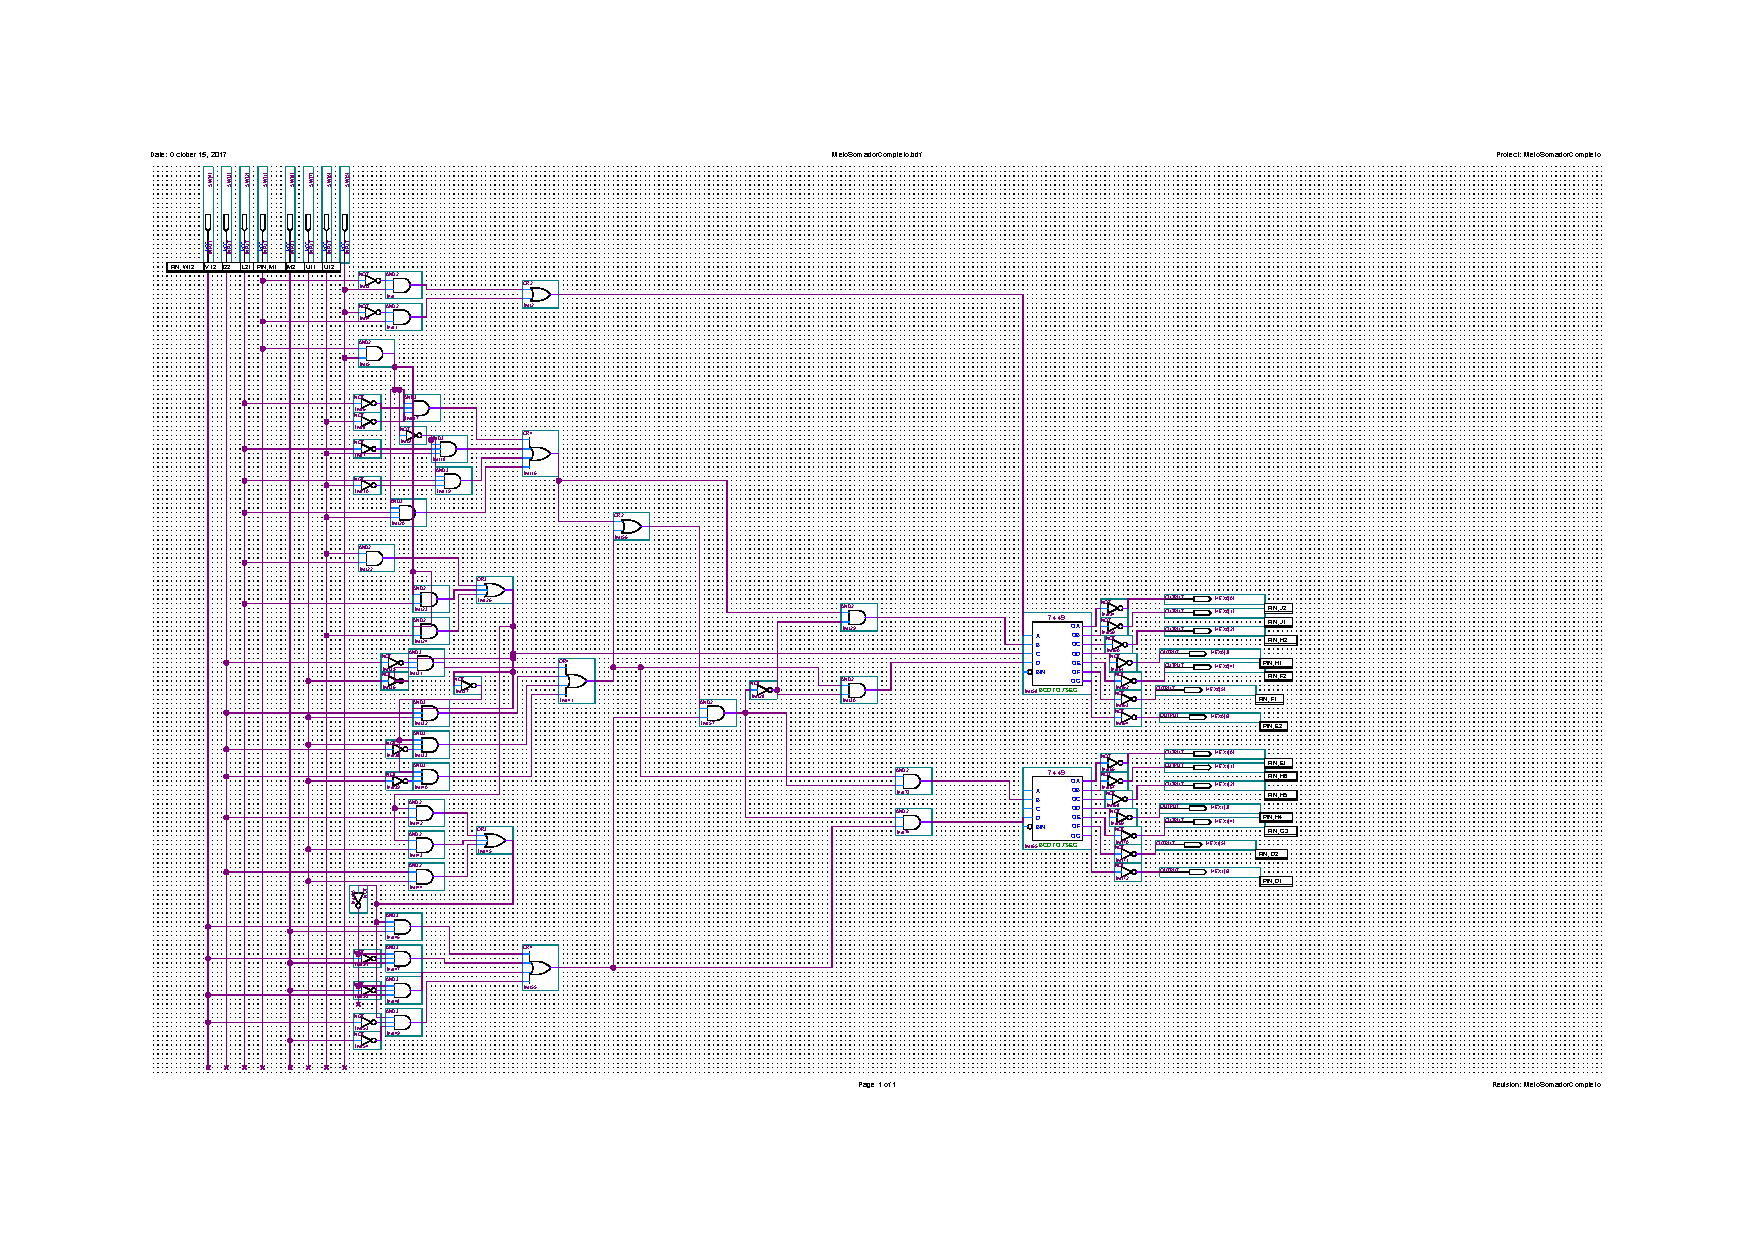
\includepdf[pages=1,landscape,frame=false]{apendices/MeioSomadorCompleto.pdf}



\end{apendicesenv}
% ---
